\section{Experiment}
In this section, we evaluate the effectiveness of our proposed framework through comprehensive experiments. 
First, we present the experimental settings, including details about the datasets, compared baselines, evaluation metrics, and the parameter configurations. Then, we report the main experimental results, highlighting the performance of the proposed framework compared with various baseline methods.
Finally, we analyze the contributions of individual model components and the impact of parameters used in our framework. We also assess the generalizability of K-RagRec in the zero-shot setting. We present the generalizability study in Appendix~\ref{appendix:General}.



\subsection{\textbf{Experimental Settings}}
\subsubsection{\textbf{Datasets}}\label{datasets}
To evaluate the performance of our K-RagRec framework, we adopt three real-world datasets.
\textbf{MovieLens-1M}\footnote{https://grouplens.org/datasets/movielens/1m/} is a dataset containing approximately one million movie ratings and textual descriptions of movies (i.e., “title”). 
\textbf{MovieLens-20M}\footnote{https://grouplens.org/datasets/movielens/20m/} is a large-scale movie ratings dataset encompassing over 20 million ratings from more than 138,000 users on 27,000 movies.
\textbf{Amazon Book}\footnote{https://jmcauley.ucsd.edu/data/amazon/} is a book recommendation dataset that records more than 10 million user ratings of books and the titles of the books.
In addition, we adopt the popular knowledge graph \textit{Freebase}\footnote{https://developers.google.com/freebase} and filter out the triples related to the three datasets to reconstruct the KG. The statistics of these three datasets and KG are presented in Table~\ref{tab:datasets}. 



% & \# Entities &  & 1,278,544 & 1,378,445 \\
%           & \# Relations &     & 508    & 753 \\






\subsubsection{\textbf{Baselines}}\label{baseline}

In the realm of LLM-based recommendation research, our work pioneers the investigation of retrieving knowledge from KGs to enhance the recommendation capabilities of LLMs.
Therefore, to evaluate the effectiveness, we compare our proposed framework with a series of meticulously crafted KG RAG-enhanced LLM recommendation baselines.
We first include two typical inference-only methods Retrieve-Rewrite-Answer~\citep{wu2023retrieve} (KG-Text) and KAPING~\citep{baek2023knowledge}, where the former retrieves sub-graphs and textualizes them, and the latter retrieves triples.
We exclude some knowledge reasoning path-based approaches~\citep{luo2023reasoning}, as it is difficult to retrieve faithful knowledge reasoning paths solely from the user's interaction items.
Next, we compare K-RagRec with various prompt-tuning approaches augmented by retrieval, including Prompt Tuning with KG-Text (PT w/ KG-Text), GraphToken~\citep{perozzi2024let} with retrieval (GraphToken w/ RAG) as well as G-retriever~\citep{he2024g}. Additionally, we evaluate our method against Lora Fine-tuning with retrieval (Lora w/ KG-Text)~\citep{hu2021lora}.



\subsubsection{\textbf{Evaluation Metrics}}
To evaluate the effectiveness of our K-RagRec framework, we employ two widely used evaluation metrics: Accuracy (ACC), and Recall@$k$ ~\citep{he2020lightgcn}. We present results for $k$ equal to 3, and 5. Inspired by recent studies~\citep{zhang2024agentcf,hou2022towards}, we adopt the \textit{leave-one-out strategy} for
evaluation. Specifically, for each user, we select the last item that the user interacted with as the target item and the 10 interaction items prior to the target item as the historical interactions. Then, we leverage LLM to predict the user's preferred item from a pool of 20 candidate items ($M = 20$), which contains one target item with nineteen randomly sampled items. For trained models (including prompt tuning and fine-tuning), we compute Recall@$k$ by extracting the probability assigned to each item and evaluating the model's ability to rank the target item within the top-$k$ predictions. In addition, we also conduct comparison experiments with 10 candidate items ($M = 10$) as shown in Appendix~\ref{appendix:10samples}.





\begin{table*}[t]
\centering
\vskip -0.150in
  \caption{Performance comparison of different KG RAG-enhanced LLM recommendations. 
  The \colorbox{backred!50}{best performance} and the \colorbox{backblue!75}{second-best performance} are marked in red and blue, respectively. ACC and R@$k$ denote
Accuracy and Recall@$k$, respectively.}
  \vskip -0.05in
    \scalebox{0.6}
{
  \begin{adjustbox}{}
    \begin{tabular}{c|c|c|c|c|c|c|c|c|c|c|c}
 %   \toprule
    \toprule
    \toprule
    \multirow{2}{*}{Models}  & \multicolumn{2}{c|}{\multirow{2}{*}{Methods}} & \multicolumn{3}{c|}{MovieLens-1M}  & \multicolumn{3}{c|}{MovieLens-20M} & \multicolumn{3}{c}{Amazon Book} \\
    \cmidrule{4-12}
    & \multicolumn{2}{c|}{} & \multicolumn{1}{c|}{ACC} & \multicolumn{1}{c|}{R@3} & \multicolumn{1}{c|}{R@5}& \multicolumn{1}{c|}{ACC} & \multicolumn{1}{c|}{R@3} & \multicolumn{1}{c|}{R@5} & \multicolumn{1}{c|}{ACC} & \multicolumn{1}{c|}{R@3} & \multicolumn{1}{c}{R@5} \\
\midrule
    \multirow{10}{*}{\textbf{LLama-2}}&   \multirow{2}{*}{\textbf{Inference-only}} 
    & KG-Text~\citep{wu2023retrieve}& 0.076  & - & -  & 0.052 &  - &  -  &  0.058  &  -  &  -   \\
    & &KAPING~\citep{baek2023knowledge} & 0.079  & -  & - & 0.069 &  - &  -  & 0.063  &   - &   -  \\
    \cmidrule{2-12}
    &\multirow{5}{*}{\textbf{Frozen LLM w/ PT}} &PT w/ KG-Text& 0.078  & 0.191  & 0.308 &0.051  &0.152 &0.250   &0.074   &0.165   &0.245   \\
    & &GraphToken w/ RAG~\citep{perozzi2024let} & 0.268  &  0.421 & 0.466 & 0.186 &0.433 &0.576   &0.326   & 0.515  & 0.624   \\
    & &G-retriever~\citep{he2024g} &  0.274 & 0.532  & 0.650 & 0.342 &0.619  &0.739   &0.275   &0.487   &0.612 \\
     & & K-RagRec & \colorbox{backblue!75}{0.435}  &  \colorbox{backblue!75}{0.725} & 0.831 &0.600  & \colorbox{backblue!75}{0.850} & \colorbox{backblue!75}{0.913}  &  \colorbox{backblue!75}{0.508}  & \colorbox{backblue!75}{0.690}  &  \colorbox{backblue!75}{0.780} \\
    \cmidrule{3-12}
    && \cellcolor{verylightgray} \textbf{Improvement} & \cellcolor{verylightgray}58.6\%  & \cellcolor{verylightgray}33.0\% & \cellcolor{verylightgray}27.8\%  & \cellcolor{verylightgray}75.4\% &  \cellcolor{verylightgray}37.3\% &  \cellcolor{verylightgray}23.5\%  &  \cellcolor{verylightgray}55.8\%  & \cellcolor{verylightgray}34.0\%   &  \cellcolor{verylightgray}25.0 \%  \\
    \cmidrule{2-12}
    &\multirow{3}{*}{\textbf{Fine-tuning}} &Lora w/ KG-Text&    0.402 & 0.718 & \colorbox{backblue!75}{0.833} &\colorbox{backblue!75}{0.609} &0.848   &0.905   &0.446   &0.648  &0.758 \\
    % \cmidrule{2-11}
     & & Lora w/ K-RagRec &  \colorbox{backred!50} {0.466} & \colorbox{backred!50} {0.770}  & \colorbox{backred!50} {0.863} & \colorbox{backred!50} {0.637}  & \colorbox{backred!50} {0.872} & \colorbox{backred!50} {0.927}  & \colorbox{backred!50} {0.516}   & \colorbox{backred!50} {0.720}   & \colorbox{backred!50} {0.799} \\
     \cmidrule{3-12}
    && \cellcolor{verylightgray} \textbf{Improvement} &  \cellcolor{verylightgray}15.9\%  & \cellcolor{verylightgray}7.2\% & \cellcolor{verylightgray}3.6\%  & \cellcolor{verylightgray}4.5\% &  \cellcolor{verylightgray}2.7\% &  \cellcolor{verylightgray}2.4\%  &  \cellcolor{verylightgray}15.7\%  & \cellcolor{verylightgray}11.1\%   &   \cellcolor{verylightgray}5.4\%    \\
   \midrule
    \multirow{10}{*}{\textbf{LLama-3}}&   \multirow{2}{*}{\textbf{Inference-only}} & KG-Text~\citep{wu2023retrieve}& 0.095  & - & -  & 0.060 &  - &  -  &  0.054  &  -  &  - \\
    & &KAPING~\citep{baek2023knowledge}& 0.084  & - & -  & 0.069 &  - &  -  & 0.062   &  -  &  - \\
    \cmidrule{2-12}
    &\multirow{5}{*}{\textbf{Frozen LLM w/ PT}} &PT w/ KG-Text& 0.134  & 0.294  & 0.433 &0.094  &0.205 &0.296   &0.083   &0.207   &0.314   \\
    & &GraphToken w/ RAG~\citep{perozzi2024let} & 0.355  & 0.622  & 0.737 & 0.473 &0.719 & 0.805  &0.428   &0.567   &0.661    \\
    & &G-retriever~\citep{he2024g} & 0.352  & 0.632  & 0.746 & 0.502 &0.736 & 0.796  &0.417   & 0.584  &0.682 \\
     & & K-RagRec & \colorbox{backblue!75}{0.472}  & \colorbox{backblue!75}{0.704}  & \colorbox{backblue!75}{0.765} &0.634  &\colorbox{backblue!75}{0.779} &\colorbox{backblue!75}{0.818}    & \colorbox{backblue!75}{0.514}  & \colorbox{backblue!75}{0.662}  & \colorbox{backblue!75}{0.723} \\
  \cmidrule{3-12}
    && \cellcolor{verylightgray} \textbf{Improvement} &  \cellcolor{verylightgray}32.9\%  & \cellcolor{verylightgray}11.4\% & \cellcolor{verylightgray}2.5\%  & \cellcolor{verylightgray}26.3\% &  \cellcolor{verylightgray}5.8\% &  \cellcolor{verylightgray}1.6\%  &  \cellcolor{verylightgray}20.0\%  & \cellcolor{verylightgray}13.4\%   &   \cellcolor{verylightgray}6.0\%     \\
    \cmidrule{2-12}
    &\multirow{3}{*}{\textbf{Fine-tuning}} &Lora w/ KG-Text& 0.449  & 0.694  &0.750 &\colorbox{backblue!75}{0.648}  &0.757 &0.790   &0.490   &0.638   & 0.698 \\
    % \cmidrule{2-11}
     & & Lora w/ K-RagRec &  \colorbox{backred!50} {0.498} & \colorbox{backred!50} {0.712}  & \colorbox{backred!50} {0.771} & \colorbox{backred!50} {0.674}  & \colorbox{backred!50} {0.786} & \colorbox{backred!50} {0.817}  & \colorbox{backred!50} {0.546}   & \colorbox{backred!50} {0.672}   & \colorbox{backred!50} {0.733}  \\
    \cmidrule{3-12}
    && \cellcolor{verylightgray} \textbf{Improvement} &   \cellcolor{verylightgray}10.9\%  & \cellcolor{verylightgray}2.6\% & \cellcolor{verylightgray}2.8\%  & \cellcolor{verylightgray}4.0\% &  \cellcolor{verylightgray}3.8\% &  \cellcolor{verylightgray}3.4\%  &  \cellcolor{verylightgray}11.4\%  & \cellcolor{verylightgray}5.3\%   &   \cellcolor{verylightgray}5.0\%      \\
   \midrule
    \multirow{10}{*}{\textbf{QWEN2}}&   \multirow{2}{*}{\textbf{Inference-only}} & KG-Text~\citep{wu2023retrieve}&0.160   & - & -  & 0.174 &  - &  -  &  0.194  &  -  &  - \\
    & &KAPING~\citep{baek2023knowledge}& 0.196  & - & -  & 0.208 &  - &  -  &  0.220  &  -  &  - \\
    \cmidrule{2-12}
    &\multirow{5}{*}{\textbf{Frozen LLM w/ PT}} &PT w/ KG-Text& 0.190 &  0.371 & 0.499 &0.259  &0.397 &0.494   &0.303   &0.451   &0.553   \\
    & &GraphToken w/ RAG~\citep{perozzi2024let} & 0.259	& 0.487	& 0.608  & 0.370 &0.550 &0.632   & 0.365  &0.568   &  0.658  \\
    & &G-retriever~\citep{he2024g} & 0.304	&0.551	&0.644  &0.389  &0.606 &0.685   &0.355   &0.552   &0.658 \\
     & & K-RagRec &   \colorbox{backblue!75}{0.416}	&\colorbox{backblue!75}{0.712}	&\colorbox{backblue!75}{0.829}  &0.586  &\colorbox{backblue!75}{0.842}  &0.904   & \colorbox{backblue!75}{0.502}  & \colorbox{backblue!75}{0.686} &  \colorbox{backblue!75}{0.767} \\
         \cmidrule{3-12}
    && \cellcolor{verylightgray} \textbf{Improvement} &   \cellcolor{verylightgray}36.8\%  & \cellcolor{verylightgray}29.2\% & \cellcolor{verylightgray}28.4\%  & \cellcolor{verylightgray}50.6\% &  \cellcolor{verylightgray}38.9\% &  \cellcolor{verylightgray}32.0\%  &  \cellcolor{verylightgray}37.5\%  & \cellcolor{verylightgray}20.8\%   &  \cellcolor{verylightgray}16.6 \%      \\
    \cmidrule{2-12}
    &\multirow{3}{*}{\textbf{Fine-tuning}} &Lora w/ KG-Text&   0.400	&0.701	&0.815  &\colorbox{backblue!75}{0.601}  &\colorbox{backblue!75}{0.842} & \colorbox{backblue!75}{0.906}  &0.478   &0.667   &0.751 \\
    % \cmidrule{2-11}
     & & Lora w/ K-RagRec &   \colorbox{backred!50} {0.466}	& \colorbox{backred!50} {0.763}	&\colorbox{backred!50} {0.860}  & \colorbox{backred!50} {0.631}  & \colorbox{backred!50} {0.868}  & \colorbox{backred!50} {0.928}   & \colorbox{backred!50} {0.510}  & \colorbox{backred!50} {0.704}  & \colorbox{backred!50} {0.780} \\
    \cmidrule{3-12}
    && \cellcolor{verylightgray} \textbf{Improvement} &   \cellcolor{verylightgray}16.5\%  & \cellcolor{verylightgray}8.8\% & \cellcolor{verylightgray}5.5\%  & \cellcolor{verylightgray}5.0\% & \cellcolor{verylightgray}3.1 \% &  \cellcolor{verylightgray}2.4\%  &  \cellcolor{verylightgray}6.7\%  & \cellcolor{verylightgray}5.5\%   &   \cellcolor{verylightgray}3.9\%      \\
    \bottomrule
    \bottomrule
    %\bottomrule
    \end{tabular}%
    \end{adjustbox}
}
  \label{tab:results}%
  % \vskip -0.16in
\end{table*}%




\subsubsection{Parameter Settings}
We implement the framework on the basis of PyTorch and conduct the experiments on 2 NVIDIA A6000-48GB GPUs. We adopt the SentenceBert to encode entities, relations, and query attributes. 
We use the 3 layers Graph Transformer as the $\text{GNN}^{\text{Indexing}}$ and $\text{GNN}^{\text{Encoding}}$ for MovieLens-1M and 4 layers for MovieLens-20M and Amazon Book. The layer dimension is set to 1024, and the head number is set to 4. 
The popularity selective retrieval policy threshold $p$ is set to 50\%.
For each item that needs to be retrieved, we retrieve the top-3 most similar sub-graphs. The re-ranking knowledge sub-graph number $N$ is set to 5. More experiment details are shown in Appendix~\ref{appendix:hyper}. We also present
several prompt examples in Appendix~\ref{appendix:prompt}.





\subsection{\textbf{Overall Performance Comparison}}
We compare the recommendation performance of K-RagRec with various baselines on three open-source backbone LLMs: LLama-2-7b~\citep{touvron2023llama}, LLama-3-8b~\citep{dubey2024llama}, and QWEN2-7b~\citep{yang2024qwen2}. We present the results in Table~\ref{tab:results}. From the comparison, we have the following main observations:
\vspace{-0.1in}
 \begin{itemize} [leftmargin=*] 
\setlength{\itemsep}{0pt}
\setlength{\parsep}{0pt}
\setlength{\parskip}{0pt}
\item Naively retrieve KG and augment LLM with text methods (i.e., KG-Text and KAPING),  have limited recommendation accuracy on the MovieLens-1M and MovieLens-20M and Amazon Book datasets.

\item Compared to other prompt tuning RAG methods, K-RagRec with LLama-2-7B as the backbone LLM leads to an average of 41.6\% improvement over the sub-optimal baseline across all datasets. With LLama-3-8B and QWEN2-7B as the backbone LLM, K-RagRec also brought an average of 13\% to 32\% improvement, highlighting the effectiveness of our proposed method in augmenting LLMs' recommendation performance.

\item Compared to the LoRA fine-tuning with the naive RAG approach, K-RagRec with prompt tuning achieves close to or better performance in most settings. Notably, K-RagRec achieves the best performance when fine-tuned with LoRA.
\end{itemize}



% \vskip -0.13in


\begin{figure}[t]
\vskip -0.1in
\centering
\subfigure[ML1M ACC]{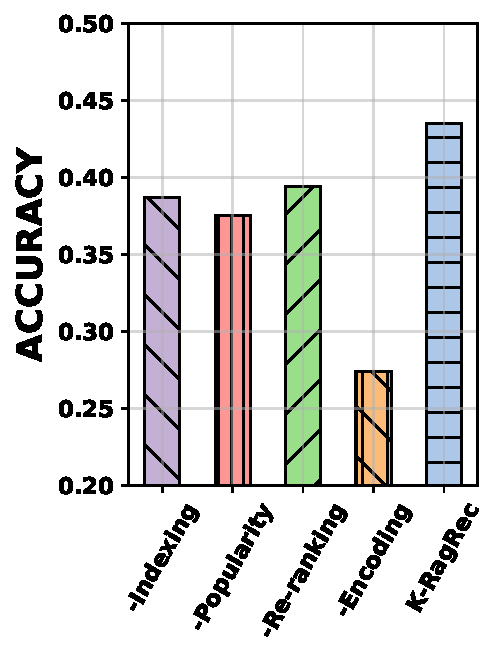
\includegraphics[width=0.32\columnwidth]{figures/ablation/ml1m-acc.pdf}}
\subfigure[ML1M R@3]{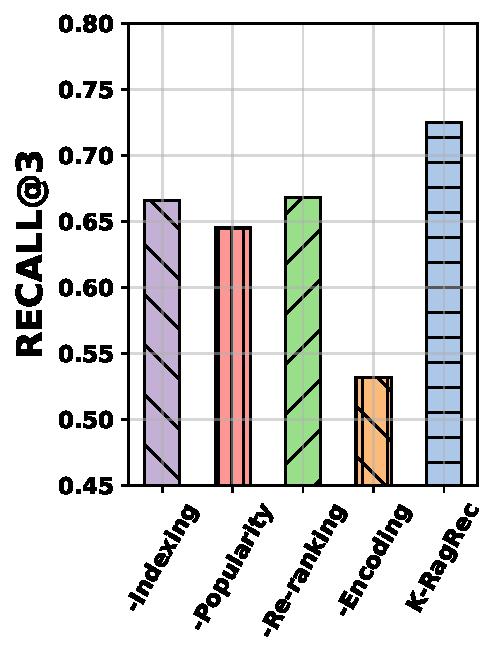
\includegraphics[width=0.32\columnwidth]{figures/ablation/ml1m-recall3.pdf}}
\subfigure[ML1M R@5]{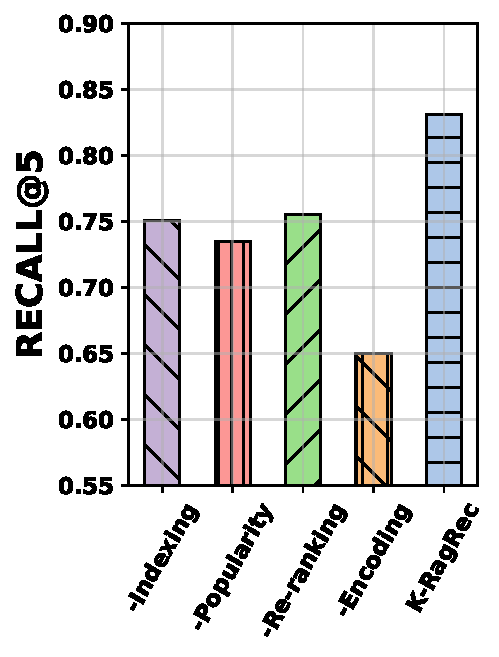
\includegraphics[width=0.32\columnwidth]{figures/ablation/ml1m-recall5.pdf}}
\subfigure[BOOK ACC]{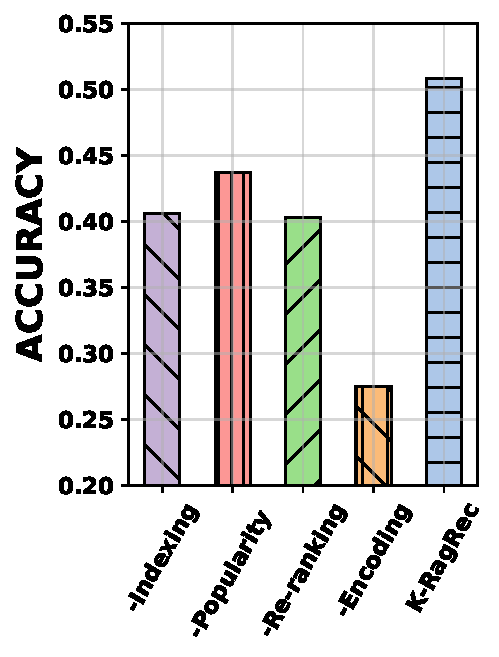
\includegraphics[width=0.32\columnwidth]{figures/ablation/books-acc.pdf}}
\subfigure[BOOK R@3]{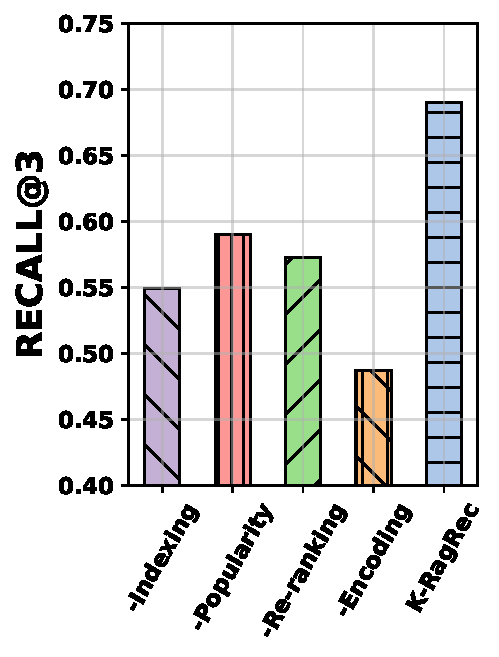
\includegraphics[width=0.32\columnwidth]{figures/ablation/books-recall3.pdf}}
\subfigure[BOOK R@5]{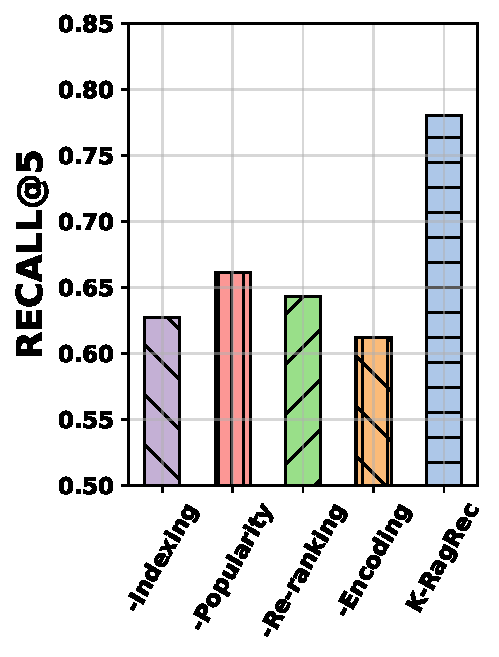
\includegraphics[width=0.32\columnwidth]{figures/ablation/books-recall5.pdf}}
% \vskip -0.13in
\caption{Comparison among K-RagRec and its four ablated variants on MovieLens-1M and Amazon Book datasets and LLama-2-7b across metrics Accuracy, Recall@3 and Recall@5.}\label{fig:ablation}
% \vskip -0.25in
\end{figure}

\subsection{\textbf{Ablation Study}}
To evaluate the impact of each component in our proposed framework, we conduct the ablation study to compare the K-RagRec with four ablated variants on MovieLens and Amazon Book datasets, using LLama-2-7B as the backbone LLM. Details of each ablation variant are provided in Appendix~\ref{appendix:Abla}. The results are illustrated in Figure~\ref{fig:ablation}.
Observing the experiment results, we find that eliminating any component of the framework leads to a decrease in the overall performance of the recommendations, demonstrating the effectiveness of each module. Secondly, removing the GNN Encoder leads to a 37\% decrease and a 45.9\% decrease in the accuracy of the model on MovieLens and Amazon Book datasets, respectively, highlighting the significance of employing GNN to encode the structure of knowledge sub-graphs. Refer to Appendix~\ref{appendix:Abla} for more details.




\begin{table}[t]
  % \vskip -0.05in
  \centering
  \caption{ 
   Comparison of the inference efficiency on the MovieLens-1M dataset and LLama-2-7b in seconds (s). ACC denote Accuracy.}
  \vskip -0.05in
    \scalebox{0.72}
{
  % \begin{adjustbox}{}
    \begin{tabular}{c|c|c}
    \toprule
    \toprule
    \multirow{1}{*}{Methods}  & \multirow{1}{*}{ACC} & \multirow{1}{*}{Time (s)}  \\
    \midrule
    w/o RAG & - & 0.92 \\
    KG-Text  & 0.076 & 2.19 \\
    KAPING & 0.079 & 6.47 \\
    GraphToken w/ RAG & 0.268 & 3.14 \\
    G-retriever & 0.274 & 5.86 \\
    \midrule
    K-RagRec & 0.429 & 1.06 \\
    \bottomrule
    \bottomrule
    \end{tabular}%
    %\end{adjustbox}
}
  \label{tab:time}%
  \vskip -0.18in
\end{table}%







\subsection{\textbf{Efficiency Evaluation}}
In this sub-section, we evaluate the inference efficiency of our proposed K-RagRec framework compared with baselines on the MovieLens-1M dataset and LLama-2-7b.
We record the time cost for one inference utilizing two NVIDIA A6000-48G GPUs. The time cost for a single inference is reported in Table~\ref{tab:time}.
By observing the experimental results, we notice that various KG RAG approaches significantly increase the inference time, which is due to the large scale of the KG. In contrast, K-RagRec achieves the best computational efficiency compared to various KG RAG methods and is only about 0.1s slower than direct inference without retrieval.
These findings highlight the efficiency of K-RagRec and validate the effectiveness of our popularity selective retrieval policy.





\subsection{\textbf{Parameter Analysis}}
In this section, we evaluate the impact of three main hyper parameters of K-RagRec, namely popularity selective retrieval policy threshold $p$, retrieved knowledge sub-graph numbers $K$,
and re-ranking knowledge sub-graph numbers $N$.
In addition, we analyze the impact of various GNN encoder variants and different GNN layer numbers for the proposed framework in Appendix~\ref{appendix:gnn encoder} and ~\ref{appendix:gnn layer}.

\textbf{1) Impact of popularity selective retrieval policy threshold $p$}:
To understand how the popularity selective retrieval policy threshold $p$ affects K-RagRec, we conduct experiments on MovieLens-1M and LLama-2-7b across two metrics. Results are shown in Figure~\ref{fig:para1}.
As the threshold $p$ increases, the recommendation performance initially improves and then decreases. When the threshold $p$ is set to a small value, only a few items are augmented. This leads to insufficient retrieval and poor recommendation accuracy. When $p$ is set to a larger value, more items are retrieved for augmentation. However, due to the re-ranking sub-graph numbers $N$ being fixed, some retrieved cold-start item knowledge sub-graphs are discarded or ranked at the back of the list, resulting in sub-optimal recommendation performance. 
On the other hand, as observed in Figure~\ref{fig:para1} (c), the inference time increases almost linearly with threshold $p$. Therefore, selecting an appropriate threshold $p$ is crucial to balance the performance and inference time.

\textbf{2) Impact of retrieved knowledge sub-graph numbers $K$ and re-ranking sub-graph numbers $N$}:
In this part, we analyze the impact of two key hyper parameters, which are retrieved knowledge sub-graph numbers $K$ and re-ranking sub-graph numbers $N$. First, to measure the impact of $K$, we perform experiments on the MovieLens dataset and fix $p=50\%, \ N=5$. As shown in Figure~\ref{fig:parak}, some relevant knowledge sub-graphs may be overlooked when $K=1$. On the other hand, larger values of $K$ can introduce irrelevant information. Therefore, we set $K$ equal to 3 in our experiments. Next, we evaluate the effect of $N$ by fixing $p=50\%$ and $ \ K=3$, and present the results in Figure~\ref{fig:paraK}. We observe that setting $N$ to between 5 and 7 results in improved performance on the Amazon Book dataset.
In general, it is important to carefully choose $K$ and $N$ based on the scale of the dataset and the KG.
